\documentclass{beamer}
\usepackage[utf8]{inputenc}
\usepackage{amsmath}
\usepackage{amsfonts}
\usepackage{amssymb}
\usepackage{graphicx}
\usepackage[absolute,overlay]{textpos}
\usepackage{geometry}
\usepackage{beamerposter}
\usepackage{multicol}
\usepackage{xcolor}

\usetheme{Berlin}
\paperwidth=48in
\paperheight=36in
\setlength{\TPHorizModule}{1in}
\setlength{\TPVertModule}{1in}
\setbeamertemplate{bibliography item}{\insertbiblabel}
\bibliographystyle{abbrv}

% Format Commands
\newcommand{\lr}[1]{\left(#1\right)}
\newcommand{\lrsq}[1]{\left[ #1 \right]}
\newcommand{\lra}[1]{\left\langle #1 \right\rangle}
\newcommand{\lrfrac}[2]{\left(\frac{#1}{#2}\right)}
\newcommand{\lrsqfrac}[2]{\left[\frac{#1}{#2}\right]}
%\newcommand{\ie}{i.e.\ }
%\newcommand{\eg}{e.g.\ }
%\newcommand{\cf}{cf.\ }
%\newcommand{\viz}{\textit{viz.}\ }
\newcommand{\needref}{\textcolor{red}{[REF]}~}

% Functions %
\newcommand{\psih}{\hat{\psi}}
\newcommand{\xbdy}{x_{bdy}(y)}
\newcommand{\besj}[2]{J_{#1}\lr{#2}}
\newcommand{\besi}[2]{I_{#1}\lr{#2}}

% Symbols %
\newcommand{\reals}{\mathbb{R}}
\newcommand{\complexes}{\mathbb{C}}
\newcommand{\muo}{\mu_{0}}

\begin{document}
\begin{frame}[t]
\begin{textblock}{30}(.5,.8)
\fontsize{72}{60}\selectfont Exploring the formation and robustness of partially relaxed MHD states
\end{textblock}
\begin{textblock}{24}(37.5,0)

\includegraphics[scale=.1]{uofwa.png}
\end{textblock}
\begin{textblock}{24}(40.6,2.3)

\includegraphics[scale=1]{pppl.png}
\end{textblock}
\begin{textblock}{24}(43.5,.9)

\includegraphics[scale=.1]{doe_logo.png}\break
\end{textblock}



\begin{textblock}{28}(.75,2.2)
{\huge
    M. Ketkaroonkul\textsuperscript{1},
    A. Wright\textsuperscript{2}
}
\end{textblock}
\begin{textblock}{24}(.75,3)
{\large
    \textsuperscript{1}University of Washington, Seattle,
    \textsuperscript{2}Princeton Plasma Physics Laboratory
}
\end{textblock}

\begin{textblock}{15}(.5,3.5)
\begin{block}{Introduction}
Multiregion Relaxed MHD (MRxMHD) is a model proposed to account for resistive effects in fusion plasmas
\begin{itemize}
    \item Ideal interfaces, or current sheets partitioning plasma regions undergoing Taylor Relaxation 
    \item Critical tool for optimizing stellarator design
    \item Model magnetic field perturbations in tokamaks
    \item {\bf Motivation --} testing the robustness of ideal interfaces, a central assumption of the model 
\end{itemize}
\end{block}

\begin{block}{Mathematical Methods}
To test the robustness of ideal interfaces, which are assumed to persist in resistive plasmas,
\begin{itemize}
    \item Application of mathematical methods -- Boundary Layer Theory, Perturbation Methods, Fourier Analysis
    \item Deriving equations from Dewar et al. (2017), Hahm and Kulsrud (1985)
    \item Analyzing Alfven $\tau_A$ and Resistivity $\tau_R$ timescales \cite{wangbhattacharjee}
\end{itemize}
\end{block}

\begin{block}{Hahm-Kulsrud-Taylor Beltrami Slab Model}
Dewar et al. (2017) presents the following model for MRxMHD in a toroidal cross-section:
A thin annular section of a toroidal cross-section transformed into Cartesian coords. \cite{dewar2017} (see figure 1a.)
The ansatz is significant in deriving the general solution to explore nonlinear vs. linear effects of a boundary perturbation.
\begin{itemize}
    \item x-axis --- radial direction of toroidal cross-section
    \item y-axis --- poloidal direction. Periodic. $y \in [-\pi,\pi]$
\end{itemize}

\begin{equation}
    \begin{split}
        \hat{\psi}_+ (x,y) & = \textcolor{red}{c_0}\cos{\mu x} + \sum_{l=1}^{\infty} \textcolor{red}{c_{l}} \cos{\frac{lmy}{a}} \cosh{\kappa_{lm} x} \\
                           & + \textcolor{red}{d_0} \sin{\mu x} + \sum_{l=1}^{\infty} \textcolor{red}{d_{l}} \cos{\frac{lmy}{a}} \sinh{\kappa_{lm} x}
    \end{split}
\end{equation} 
where

\begin{itemize}
    \item \begin{equation}
                k_l = \pm i \kappa_l = \sqrt{\left({\frac{lm}{a}}\right)^2 - \mu^2}
    \end{equation}
\item $\psi=\overline{\psi} + \frac{\overline{F}}{\mu} (1-\cos\mu x) + \hat{\psi}$
    \item $m$ is an integer mode multiple
    \item $a$ is the characteristic length of the slab model
    \item $c_0=-\overline{\psi},d_0=c_l=0,d_l$ to be determined

\end{itemize}

\end{block}
\end{textblock}

\begin{textblock}{15}(.5,19)
    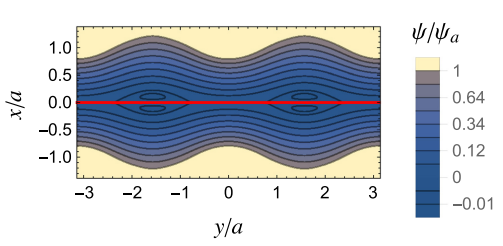
\includegraphics[scale=1]{dewar-boundary-ripples.png} 
    \newline
    1a. Slab Model as presented in Dewar et al. (2017). \cite{dewar2017}
\end{textblock}

\begin{textblock}{15}(8.75,18.5)
    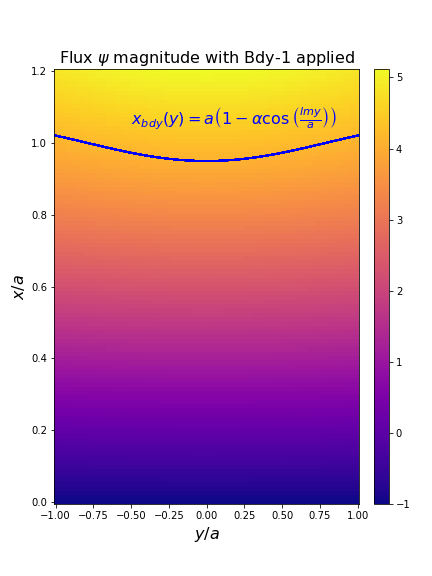
\includegraphics[scale=1.2]{bdy-1_general-solution.png} 
    \newline
    1b. Plotted flux function applying Bdy-1. \cite{dewar2017}
\end{textblock}

\begin{textblock}{15}(.5,24)
    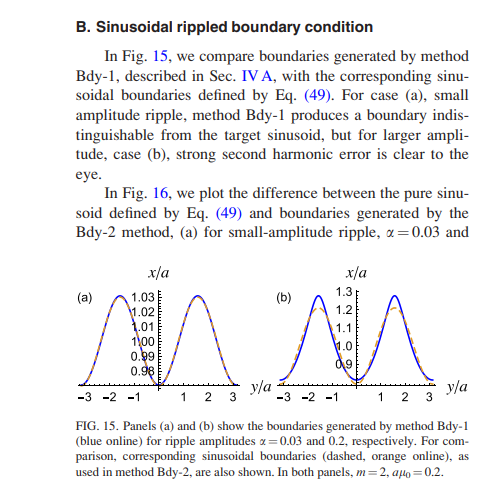
\includegraphics[scale=1]{dewar-bdy1-error.png} 
    \newline
    1c. As $\alpha$ increases, the boundary ripple from Bdy-1 deviates from the actual. \cite{dewar2017}
\end{textblock}


\break

\begin{textblock}{15}(16.5,3.5)
\begin{block}{Applying Bdy-1}
    Implicit description of boundary perturbation, accurate for small values of $\alpha$ \cite{dewar2017} (see figure 1c.)
\begin{equation}
    \label{eq:bdy1}
    \psi\left( \pm a, y \right) - \langle \psi\left( \pm a, y \right) \rangle = 2\alpha \psi_a \cos{\frac{lmy}{a}}
\end{equation} 
where
\begin{itemize}
    \item $\psi_a$ -- magnetic flux at the ripple boundary
    \item $\alpha$ -- amplitude of boundary ripple (small value)
\end{itemize}
\newline
which yields the solution
\begin{equation}
\begin{split}
    \hat{\psi}_+ (x,y) & = -\overline{\psi}\cos{\mu x} \\
                       & + \frac{2\alpha \psi_a}{\sinh{\kappa_1 a}} \sinh{\kappa_1 x} \cos\left( \frac{my}{a} \right) \\
                       & + \frac{2\alpha \psi_a \gamma_s \kappa_1}{\mu \sinh\left( \kappa_1 a \right) } \sin\left( \mu x \right) 
\end{split}
\end{equation}
\begin{itemize}
    \item $\gamma_s$ -- dimensionless parameter
\end{itemize}
\end{block}

\begin{block}{Applying Bdy-2}
    Explicit description of rippled boundary \cite{dewar2017}
\begin{itemize}
    \item accurate for a greater range of $\alpha$ 
    \item Solution is more sophisticated -- used Taylor expansion approximation for terms $\sim O(\alpha^2)$ and expansion of Bessel Functions
\end{itemize}
\begin{equation}
    \label{eq:bdy2}
    x_{\text{bdy}}\left( y \right) =a\left( 1-\alpha\cos{\frac{lmy}{a}} \right) 
\end{equation} 
\end{block}

\begin{block}{Taylor Expansion Approximation of Bdy-2}
\begin{equation}
    \textcolor{red}{d_0}=\frac{1}{\sin{\mu a}} \lr{\psi_a - \lr{\overline{\psi} + \frac{\overline{F}}{\mu}}(1-\cos{\mu a})}
\end{equation} 
\begin{equation}
    \textcolor{red}{d_1}=\frac{\mu a \alpha}{\sinh{\kappa_1 a}}\lr{d_0\cos{\mu a} + \lr{\frac{\overline{F}}{\mu}    + \overline{\psi}}\sin{\mu a}}
\end{equation} 

where
\begin{itemize}
    \item $\overline{F}$ -- mean toroidal flux, which is much stronger than poloidal flux
    \item $\overline{\psi}$ -- mean poloidal flux
\end{itemize}

\end{block}
\begin{block}{Bessel Function Solution of Bdy-2}
The following equation describes a simultaneous system of equations
\begin{multline}
    \frac{\textcolor{red}{d_p}}{2}\sinh\lr{\kappa_p a}\besi{0}{\kappa_p a \alpha}+\sum_{l=1}^{\infty}\textcolor{red}{d_l}\lrsq{\sinh\lr{\kappa_l a}-\cosh\lr{\kappa_l a}}\besi{l-p}{\kappa_l a \alpha}\\
    = -\textcolor{red}{d_0}\left[i^{p+1}e^{-i\mu a}\besj{p}{\mu a \alpha}\right]-\frac{i^p e^{-i\mu a}\lra{F_0}}{\mu}\besj{p}{\mu a \alpha},\label{eq2.42}
\end{multline}
\begin{itemize}
    \item $p$ is a mode number which can vary to form the system of equations. By truncating the series with index $l$, we can vary $p$ to account for the system of equations for the coefficients
\end{itemize}
    
\end{block}

\begin{block}{MHD Equation Models}
    The following equations presented in Hahm and Kulsrud (1985) are the MHD equations that will be used to test the assumptions of MRxMHD against \cite{hahmkulsrud}. The general solution derived from Dewar et al. will be tested in these MHD equations.
\begin{equation}
    \label{eq:hk15}
    \frac{\partial \psi}{\partial t} + \vec{V}\cdot \vec{\nabla} \psi= \frac{\eta}{\mu_0} \nabla ^2 \psi
\end{equation} 
\begin{equation}
    \label{eq:hk16}
    \rho\left( \frac{\partial }{\partial t} + \vec{V}\cdot \vec{\nabla} \right)\omega_z = \vec{B}\cdot \vec{\nabla}j_z
\end{equation} 
where
\begin{equation}
    \vec{V}= \hat{z}\times \vec{\nabla}\phi
\end{equation} 

\begin{equation}
    \omega_z = \hat{z}\cdot \vec{\nabla}\times \vec{V}=\nabla ^{2}\phi
\end{equation}
where
\begin{itemize}
    \item $\psi$ -- magnetic flux
    \item $\phi$ -- stream function of plasma
    \item $\eta$ -- resistivity
    \item $\rho$ -- mass density
    \item $j$ -- current density
\end{itemize}

\end{block}

\end{textblock}

% \includegraphics[scale=1]{mu-test-DvsD.jpg}\includegraphics[scale=1]{mu-test-trace.jpg}


\begin{textblock}{15}(32.5,3.5)
\begin{block}{Linearization of MHD Equations via Perturbation Methods}
Using a perturbation series with a small parameter $\varepsilon$,
\begin{equation}
   \psi=\sum_{n=0}^{\infty} \varepsilon^{n}\psi_n=\psi_0+\varepsilon\psi_1+\varepsilon^{2}\psi_2+\ldots 
\end{equation}
and substituting the variables within the MHD equations, the first order equations are
\begin{equation}
    \frac{\partial \psi_1}{\partial t} -\frac{kB_0x}{a}\phi_1\left( x,t \right) = 0
\end{equation} 
\begin{equation}
    \rho \frac{\partial}{\partial t} \frac{\partial^2}{\partial \chi^2} \phi_1(x,t) &= -\frac{kB_0 \chi}{\mu_0} \left( \frac{\partial ^2}{\partial \chi^2} \psi_1 \right)
\end{equation} 
where $\chi=x / a$ and $\tau=t / \tau_A$.

    
\end{block}
\begin{block}{Timescale Evolution}
    \begin{itemize}
        \item In Wang and Bhattacharjee (1992), presented that characteristic timescales of the plasma evolution depended on $\tau_A,\tau_R$ \cite{wangbhattacharjee}
        \item $\tau_A=\sqrt{\mu_0\rho_0 a^2}/B_0$ Alfvén Timescale
        \item $\tau_R$ Resistivity Timescale
        \item $\tau=\tau_A^{(1-s)}\tau_R^s$
    \end{itemize}
\begin{center}

\begin{tabular}{|l|l|l|}
    \hline
        & $\tau_A$ (ideal) & $\tau_R$ (non-ideal) \\
    \hline
        Phase A & 2/3 & 1/3 \\
    \hline
        Phase B & 2/5 & 3/5 \\
    \hline
        Phase C & 1/2 & 1/2 \\
    \hline
        Phase D & 1/4 & 3/4 \\
    \hline
\end{tabular}
\end{center}
\end{block}

\begin{block}{Further Work}
\begin{itemize}
    \item General solution in Dewar et al.
        \begin{itemize}
            \item Comparing derivations of coefficients from Bdy-1 and Bdy-2 presented in Dewar et al. (2017)
            \item Developing coefficient solver for Bdy-2
            \item Testing the magnetic flux solution found in Dewar et al. (2017) with the linearized equations derived in Hahm and Kulsrud (1985)
        \end{itemize}
    \item Applying Boundary Layer Theory methods to study local properties of ideal interfaces
    \item MHD Equations in Hahm and Kulsrud
        \begin{itemize}
            \item Utilizing non-dimensionalization of linearized differential equations to determine hybrid characteristic timescales (a mix of Alfvén and resistivity timescales ($\tau_A$ and $\tau_R$.))
        \end{itemize}
\end{itemize}
\end{block}
\begin{block}{References}
\nocite{lazerson}
\bibliography{ref}
\end{block}
\begin{block}{Ackowledgments}
This work was made possible by funding from the Department of Energy for the Summer Undergraduate Laboratory Internship (SULI) program. This work is supported by the US DOE Contract No. DE-AC02-09CH11466.
\end{block}
\end{textblock}
\end{frame}
\end{document}
